\section {The arduino}
\begin {frame} {Outline}
    \tableofcontents [current]
\end {frame}

\begin {frame} {The micro controller development board}
    \begin {center}
    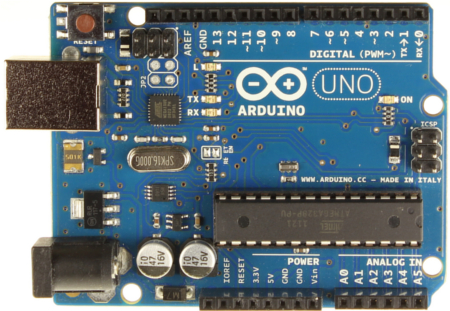
\includegraphics [width=.7\textwidth,keepaspectratio] {img/arduino}
    \end {center}
\end {frame}

\begin {frame} {The micro controller development board}
	Most of the different kinds of arduino are composed by :
	\begin{itemize}
		\item a power connector
		\pause
		\item an USB port (used as a power source and serial port)
		\pause
		\item a reset button
		\pause
		\item some leds (TX RX and pin 13 and power)
		\pause
		\item Ground, 5V and 3.3V pins
		\pause
		\item an ATmega micro controller
		\pause
		\item analog input pins (A0 to A5)
		\pause
		\item some digital pins (0 to 13)
	\end{itemize}
\end {frame}

% on remontre l'arduino en montrant les différents composants
\begin {frame} {The micro controller development board}
    \begin {center}
    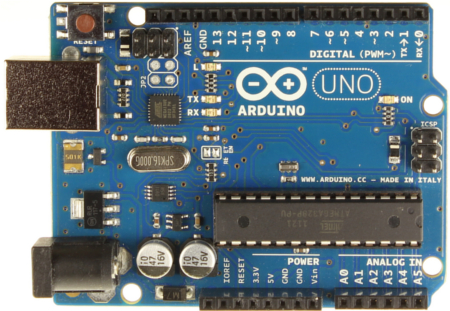
\includegraphics [width=.9\textwidth,keepaspectratio] {img/arduino}
    \end {center}
\end {frame}

